\documentclass[useAMS,usenatbib]{mn2e}
\usepackage{graphicx}
\usepackage{url}
\usepackage{tikz}
\newcommand{\aap}{Astron. Astrophys.}
\newcommand{\aj}{Astron. J.}
\newcommand{\ao}{Appl. Opt.}
\newcommand{\apj}{Astrophys. J.}
\newcommand{\apjl}{Astrophys. J. Lett.}
\newcommand{\apjs}{Astrophys. J. Suppl.}
\newcommand{\mnras}{Mon. Not. Roy. Ast. Soc.}
\newcommand{\nat}{Nature}
\newcommand{\pasa}{Publ. Ast. Soc. Aust.}
\newcommand{\pasp}{Publ. Ast. Soc. Pac.}
\newcommand{\prl}{Phys. Rev. Lett.}
\newcommand{\msun}{\mathrm{M}_\odot}

\title[E\"otv\"os Experiments]{E\"otv\"os Experiments with 
  Supermassive Black Holes  }
\author[A. Asvathaman and J. S. Heyl]{Asha Asvathaman and Jeremy S. Heyl\thanks{Email:
    heyl@phas.ubc.ca; Canada Research Chair} \\
Department of Physics and Astronomy, University of British
Columbia, 6224 Agricultural Road, Vancouver, BC V6T 1Z1, Canada}


\begin{document}
\date{Accepted ---. Received ---; in original form ---}

\pagerange{\pageref{firstpage}--\pageref{lastpage}} \pubyear{2015}

\maketitle

\label{firstpage}

\begin{abstract}
  By examining the locations of central black holes in two elliptical
  galaxies, M\,32 and M\,87, we derive constraints on the violation of
  the strong equivalence principle for purely gravitational objects,
  {\em i.e. black holes}, of less than six percent, $|\eta_N|<0.06$.
\end{abstract}

\section{Introduction}

The strong equivalence principle (SEP) states that any object
regardless of its composition will travel through a gravitational
field in the same way.  This includes objects with varying
contributions of gravitational energy.  In particular a black hole
whose mass is entirely gravitational should travel in the same manner
through the gravitational field as a
star. \citet{1968PhRv..169.1014N,1968PhRv..169.1017N} argued that
metric theories of gravity other than general relativity may exhibit
violations of the SEP --- in particular,
objects whose have a large contribution of gravitational energy to
their makeup may travel differently through a gravitational field than
other objects.

Typically the strong equivalence principle is probed by looking for
the Nordvedt effect in the Earth-Moon system or binary stars
consisting of a neutron star and a white dwarf \citep{Stairs:2005}.
The \citet{1968PhRv..170.1186N} effect results in the polarization of
an orbit in the direction of the gravitational acceleration of a large
body: the Sun in the case of the Earth-Moon system
\citep{1976PhRvL..36..551W,1976PhRvL..36..555S}, and the Galaxy in the
case binary pulsars.  The recently discovered millisecond pulsar in a
triple system, PSR J0337+1715, will provide further interesting
constraints \citep{Ransom:2014aa}.

Here we propose a new test.  In particular we will examine the
polarization of the orbits of supermassive black holes through the
central regions of elliptical galaxies.  We will focus on elliptical
galaxies because the presence of central black holes is common in
sufficiently large elliptical galaxies and the location of the centre
of the stellar potential is straightforward to constrain.
Interactions between galaxies are ubiquitous, so example systems are
straightforward to find.  In particular we will examine the small
elliptical galaxies that orbit the largest neighbour of the Milky Way
galaxy, the Andromeda galaxy or M\,31, and the massive elliptical
galaxy, M\,87, in the Virgo cluster.

\section{Calibration}

Let us suppose that we are studying a small stellar system in the
gravitational of a large one.  The stars in the small system
experience an acceleration toward the centre of the larger one
\begin{equation}
  a_\star = \frac{GM}{d^2}
  \label{eq:1}
\end{equation}
where $d$ is the distance between the small system and the larger one
and $M$ is the mass of the larger system.  These accelerations are
typically ten to one hundred times larger than those exerted by
large-scale structure $a \sim 600~\mathrm{km~s}^{-1} H_0 \sim 10^{-10}
\mathrm{cm~s}^{-2}$.

Furthermore, let us assume that the a massive black hole within the
smaller system experiences a different acceleration
\begin{equation}
  a_\bullet = \left ( 1 - \Delta \right ) a_\star
  \label{eq:2}
\end{equation}
where $\Delta$ quantifies the extent of violation of the
SEP. \citet{1982RPPh...45..631N} presents an equivalent definition
where the ratio of the inertia masses and passive gravitational mass
of an object could depend on its constitution and in particular the
contribution of gravitational energy,
\begin{equation}
  \frac{m_\mathrm{Gp}}{m_\mathrm{I}} = 1- \eta_N \frac{U_\mathrm{G}}{mc^2}.
  \label{eq:14}
\end{equation}
In the context of the parameterized post-Newtonian treatment of
deviations from general relativity \citep{Will:lrr},
\begin{equation}
  \eta_{N} =4\beta−\gamma − 3− \frac{10}{3} \xi - \alpha_1 +
  \frac{2}{3} \alpha_2 - \frac{2}{3} \zeta_1 - \frac{1}{3} \zeta_2.
\end{equation}
For the case of a black hole, $U_\mathrm{G} = mc^2$ so
$\Delta=\eta_N$. 

The massive black hole also experiences an acceleration due to the
stellar system in which it resides.  Furthermore, dynamical friction
with the less massive stars nearby damps any motion of the black hole
relative to its equilibrium position.  Near minimum of the stellar
potential we can approximate it as a harmonic oscillator so
\begin{equation}
  \left (1 - \Delta \right) \omega^2 x
   = a_\bullet - a_\star = -\Delta \frac{GM}{d^2}
  \label{eq:3}
\end{equation}
and $x$ is the displacement of the black hole from the centre of the
small stellar system in the direction of the larger system.  The value
of $\omega$ depends on the structure of the small stellar system and
depends on the mean density within the region surrounding the black
hole.  For a \citet{1990ApJ...356..359H} model
for the density distribution that well describes the stellar
distribution of elliptical galaxies
\begin{equation}
  \rho = \frac{m}{2\pi} \frac{a}{r} \frac{1}{(r+a)^3}
  \label{eq:4}
\end{equation}
where $R_\mathrm{eff}$, the half-light radius in projection is
approximately $1.8153 a$.  We take the black hole mass to be
$m_\bullet = 0.005 m$ where $m$ is the mass of the small system, we
find that
\begin{equation}
  \omega^2 \approx \frac{Gm}{a^3}
  \label{eq:5}
\end{equation}
from n-body simulations independent of the number of particles in the
simulations from 10,000 to 250,000.  In these simulations we find that
small perturbations of the black hole from the centre result in
sinusoidal oscillations with this typical frequency, regardless of the
amplitude of the perturbation (as long as its small), the number of
particles and the softening length adopted.  The half-mass radius of
the Hernquist model is $a/(\sqrt{2}-1)$ so the typical frequency
within the half-mass radius is
\begin{equation}
  \omega^2 = \frac{4\pi}{8} (\sqrt{2}-1)^3 \frac{G m}{a^3} \approx
  0.11 \frac{Gm}{a^3}.
  \label{eq:6}
\end{equation}
The oscillation frequency of the black hole is significantly larger
than the typical frequency of the system because the black hole lies
near the centre of the galaxy where typical density is larger.  On the
other hand, if one directly used Eq.~(\ref{eq:4}) to calculate the
restroring force toward the centre, one would find that it is constant
with displacement from the centre.  This would assume that the density
is actually singular at the centre but also would neglect the effect
of the black hole on the neighbouring stars which would be dragged
with it.  If we assume that the black hole lies within a bulge and
halo approximately modelled by a Hernquist model \citep[as
  in][]{1997ApJ...487..153V}, we find that
\begin{equation}
  \frac{x}{d} = 
\frac{\Delta}{1-\Delta} \frac{M}{d^3} \frac{a^3}{m},
  \label{eq:13}
\end{equation}
so the relative displacement only depends on the relative masses and
sizes of the various bodies and the angular displacement does not
depend on the distance to the systems from Earth.  We can make this
explicit by calculating the apparent displacement across the sky as
\begin{equation}
  \Delta \theta = \frac{\Delta}{1-\Delta} \frac{M}{\delta^2} \frac{\alpha^3}{m} \cos^3 i
\end{equation}
where $i$ is the inclination of the line connecting the two bodies
with respect to the plane of the sky, $\delta$ is the angular distance
between the bodies and $\alpha$ is the angular size of the Hernquist
radius $a$ of the host galaxy.  If smaller galaxies are distribution
as an isothermal distribution about the perturbing galaxy as
\citet{2006AJ....131.1405K} found for the satellites of M\,31, the
mean value of the geometric term $|\cos^3i|$ is $4/(3\pi) \approx
0.42$ and the median value is $\sqrt{2}/4\approx 0.35$.  Ninety
percent of the time the term lies between $5\times 10^{-4}$ and 0.99,
so geometric information is especially useful to give firm
constraints.  Of course the halo of the galaxy group must end
somewhere so the lower limit on $\cos^3 i$ found here is somewhat
unrealistic.  On the other hand if the density of satellites is
proportional to $r^{-3}$ like the outer regions of the
Navarro-Frenk-White profile (\citeyear{1996ApJ...462..563N}), the mean
value of the geometric term is $3\pi/16 \approx 0.59$ and the median
value is $3\sqrt{3}/8 \approx 0.65$.  Ninety percent of the time the
term lies between 0.03 and 0.996.

\section{The Andromeda Galaxy System}

The nearest neighbour of the Milky Way has four small elliptical
galaxies orbiting it: M\,32, NGC\,205, NGC\,147 and NGC\,185.
Fig.~\ref{fig:M31-system} depicts the location of the various galaxies
relative to each other from the distances compiled by
\citet{2006AJ....131.1405K}.  Of course, the distances to the various
galaxies are more uncertain than their positions on the sky.
\begin{figure}
  \begin{center}
  \begin{tikzpicture}
    \begin{scope}[scale=25]
      \draw [rotate around={-20:(0:0.774)}] (0:0.774)
      ellipse (0.005 and 0.02) node [right] {M\,31};
      \draw (-4/10:0.770) circle (0.001) node [left] {M\,32}
      (6/10:0.830) circle (0.001) node [right] {NGC\,205}
      (8:0.620) circle (0.001) node [left] {NGC\,185}
      (8:0.755) circle (0.001) node [left] {NGC\,147};
      \draw [dashed] (0:0.774) circle  (0.1);
    \end{scope}
  \end{tikzpicture}
  \end{center}
  \caption{The geometry of the largest elliptical satellite galaxies
    of the Andromeda Galaxy. The Sun is to 773~kpc to the left of
    M\,32, and the radius of the dashed circle is 100~kpc.}
  \label{fig:M31-system}
\end{figure}

A supermassive black hole (SMBH) has already been discovered in the
core of the compact elliptical galaxy M\,32
\citep{1997Natur.385..610V} and found to be within 0.5 arcseconds of
then nucleus of the galaxy \citep{2015arXiv150203231Y}.  M\,32 is
located about 0.4$^\circ$ from the centre of M\,31 in the plane of the
sky.  We can estimate the displacement of the black hole from the
centre of M\,32 as a function of $\Delta$ in the best-case scenario of
the minimal separation of M\,32 from M\,31 of about 5~kpc.  In this
case M\,32 would be well within the halo of M\,31, and we could use
the circular velocity of M31 of 240~km/s to estimate the acceleration
of M\,32 toward the centre of M31, $a_\star$ in Eq.~(\ref{eq:1}),
\begin{equation}
  a_\star = \frac{v^2}{d} = 3.7\times 10^{-8} \mathrm{cm~s}^{-2}
  \label{eq:7}.
\end{equation}
For the galaxy M\,32 we take $m=8 \times 10^8 \msun$ and
$R_\mathrm{eff} = 100$~pc so $a=55$~pc and
\begin{equation}
  x = 0.55 \frac{\Delta}{1-\Delta} \mathrm{pc}
  \label{eq:8}
\end{equation}
or
\begin{equation}
  \Delta \theta = \frac{x}{d_\mathrm{M32-Sun}} = 0.17 \frac{\Delta}{1-\Delta} \mathrm{arcseconds},
  \label{eq:9}
\end{equation}
so if M\,32 lies indeed at the close to minimum distance to M\,31, the
existing measurement of the position of the black hole yields a
constraint; either $\Delta < 0.75$ or $\Delta>1.5$.
\citet{2014ApJ...788L..38D} argue that the actual position of M\,32 is
85~kpc in front of the disk of M\,31.  Here the expected displacement
is much smaller
\begin{equation}
  x = 0.02 \frac{\Delta}{1-\Delta} \mathrm{pc}
  \label{eq:10}
\end{equation}
and only
\begin{equation} 
  \Delta \theta = \frac{x}{d_\mathrm{M32-Sun}}
  \frac{5~\mathrm{kpc}}{85~\mathrm{kpc}} = 0.0004
  \frac{\Delta}{1-\Delta} \mathrm{arcseconds}
  \label{eq:11}
\end{equation}
where we have taken the mass enclosed within the halo of M\,31 to
be $10^{12} \msun$.

We can improve upon the astrometric constraint of
\citet{2015arXiv150203231Y} if we assume that the position of the
black hole is coincident with the cusp in the surface brightness of
the galaxy.  This is a reasonable assumption because the black hole
would entrain the neighboring stars, so the stellar nucleus should be
centered on the black hole. To measure the possible deviation of the
position of the black hole on the sky and the centre of the potential
well of the galaxy we use images from the Wide-Field Camera 3 (WFC3)
on the Hubble Space Telscope (HST) in the filter, F555W.  This
instrument features 0.04~arcsecond pixels and a $162 \times
162$-arcsecond field of view.  Both the Space Telescope Imaging
Spectrograph (STIS) and the planetary camera on Wide-Field Planetary
Camera 2 (WF/PC2) feature a finer pixel scale but at the expense of
field of view.  We used images from GO-11714 (PI: Bond) with total
exposure time of 120~seconds.  To localise the core, we used circular
and elliptical apertures of 0.16 arcseconds and 0.2 arcseconds.  To
localise the centroid of the outer regions we used two elliptical
annuli: one of inner axes 2.8 and 4.3 arcseconds and outer axes of 5.7
and 8.5 arcseconds and one half that size.  The centres of the annuli
are initially roughly placed within about an arcsecond of the core and
updated to lie on the calculated centroid. This is iterated thirty
times.  The centroids of the various annuli to probe the galactic
potential coincide to within 0.01~arcseconds as do the ellipses and
circles centered on the stellar cusp, yielding an estimate of the
precision of 0.01~arcseconds.  Furthermore, the centroid of the cusp
and the outer regions also agree to within 0.01~arcseconds.  If we
combine this constraint with the distance estimate of
\citet{2006AJ....131.1405K}, this yields a constaint, $|\Delta|<
0.06$.

The three smaller elliptical galaxies, NGC\,205, NGC\,147 and NGC\,185,
have more favourable geometry and smaller mass densities.  However,
SMBHs have not yet been identified in these galaxies.  Each of these
galaxies has a mass of about $2 \times 10^8 \msun$ and a
$R_\mathrm{eff} \approx 300$~pc, so $a \approx 165$~pc.  The two
galaxies, NGC\,147 and NGC\,185 are each about 100~kpc from M31, so the
enclosed halo mass is about $10^{12} \msun$.  This yields a
typical value of the displacement of
\begin{equation}
  x = 2.3 \frac{\Delta}{1-\Delta} \mathrm{pc} ~\mathrm{and}~
  \Delta \theta = 0.75 \frac{\Delta}{1-\Delta} \mathrm{arcseconds}.
  \label{eq:12}.
\end{equation}
Although NGC\,205 may be somewhat closer to M~31 at 50~kpc than the
other galaxies, the geometry is somewhat poorer perhaps reducing the
angular displacement by a factor of two counteracting the increased
acceleration.  This yields a similar observed displacement.  If a SMBH
is discovered near the centre of these galaxies and can be localised
within 0.5~arcseconds, this would yield a constraint of $-2.0 < \Delta
< 0.4$.

On the other hand if NGC\,205 lies at the same distance from us as
M\,31, this minimum possible distance to M\,31 is about 7~kpc, and we
obtain a much larger linear and angular displacement
\begin{equation}
  x = 43. \frac{\Delta}{1-\Delta} \mathrm{pc} ~\mathrm{and}~
  \Delta \theta = 13. \frac{\Delta}{1-\Delta} \mathrm{arcseconds}.
\end{equation}
In this most favourable case the constraint would be $|\Delta| < 0.04$
with 0.5-arcsecond astromety and $|\Delta|<8\times 10^{-3}$ with
0.01-arcsecond astrometry.

\section{Virgo Elliptical Galaxies}

One of the largest elliptical galaxies in the Virgo Cluster, M\,87,
also contains a supermassive black hole and lies at the centre of the
Virgo A subcluster which contains the bulk of the mass of the Virgo
Cluster, about $10^{14} \msun$.  The Virgo Cluster is still in the
process of forming and contains at least two additional subclumps of
masses of about $10^{13} \msun$.  The subclump closest to M\,87 is
centered on M\,84 and M\,86 about $1.3^\circ$ away.  M\,89 is also a
similar angular distance away, so this analysis applies to it as well,
but it is likely to be less massive.

For the galaxy M\,87 we take $R_\mathrm{eff}=164^{\prime\prime}$
\citep{2006ApJS..164..334F} so $a=90^{\prime\prime}$.  We will take
the mass of M\,87 to be about $4\times 10^{12} \msun$
\citep{2006ApJ...643..210W} and take the mass of the subclump to be
$10^{13} \msun$ at a distance of $1.3^\circ$. This yields a
displacement of
\begin{equation}
  \Delta \theta = 0.08 \frac{\Delta}{1-\Delta} \cos^3 i
  \mathrm{arcseconds}.
  \label{eq:16}
\end{equation}
We can examine the stellar distribution of M\,87 in further detail.
\citet{2006ApJS..164..334F} find that the central region of M\,87 is
better fit by a ``core-S\'ersic'' model
\citep{1968adga.book.....S,2004AJ....127.1917T} that has a much less
cuspy central surface brightness distribution than a Hernquist model.
The break radius between the core and the outer S\'ersic model is
about 7~arcseconds.

%%%%%%%%%%%%%%%%%%%%%%%%%%%%%%%%%%%%%%%%%%%%%%%%%%%%%%%%%%%%%%%%%%%%%%%%%%%
%%
%% g-band values
%%
%% mure = 23.45, gamma = 0.322, n = 6.094, re = 163.83, rb = 7.15 
%%
%% b_n = 1.992 n - 0.3271
%%
%% one arcsecond = 80 pc
%%
%% Mg(sun) = 5.45 (Blanton et al) mg(sun)=36.5242 at M87
%%
%% 1.7e5 Lsun,g per square arcsecond
%% 26.5 Lsun,g per square parsec
%%
%% fouter at rb = 1, fouter(re) = 0.008680928977
%%
%% So the normalization is 115.1950445*26.5 Lsun = 3053 Lsun/pc^2
%%  or 1.96e7 Lsun / arcsecond^2
%%           
%%
%% In abel.dat at 1 arcsecond we have rho = 2.651419 per arcsecond
%% 5.189e7 Lsun / arcsecond^3
%% 115 Lsun / pc^3 -- 460 Msun/pc^3
%%
%% out to rb we have
%%
%% Mr = 0.113e7 Msun (r/pc)^1.638
%%
%%
%%
%%                                          5.18e-6 per (pc)^3
%%
%%
%%                        b   /   r  \1/n
%%             d log I     n  | ---- |
%% gamma_s = - ------- = ---- |  r   |
%%             d log r     n  \   e  /    
%%
%%
%%
%%
%%                  11.812148  / 7.15  \1/6.094
%% gamma_s at rb =  ---------  | ----  |    
%%                    6.094    \163.83 / 
%%
%%               =  1.938 * 0.5981571912 = 1.1592286365 >> 0.322
%%
%%
%% gamma steppens by 0.84
%%
%% within rb vcirc propto r^0.5 ... outside propto 
%% in 3-D inner profile is 1.322 switching at rb;
%% outer would be 2.1592286
%%
%% get normalization from abel.dat at 1 arcsecond
%%
%%
%% Outside rb the slope is much steeper.
%%
%%%%%%%%%%%%%%%%%%%%%%%%%%%%%%%%%%%%%%%%%%%%%%%%%%%%%%%%%%%%%%%%%%%%%%%%%%%

\citet{2013ApJ...770...86W} determine the mass of the central black
hole of M\,87 to be about $3.5 \times 10^{9} \msun$ (approximately
$10^{-3}$ of the mass of the galaxy) and to dominate the mass within
within about 5.61~arcseconds of the centre.  They also model the
contribution of the stellar mass to the circular velocity in this
inner region, yielding a value of about 160~km/s at $4^{\prime\prime}$
from the black hole consistent with the photometry of
\citet{2006ApJS..164..334F} and a mass-to-light ratio of 4. Assuming a
smaller mass-to-light ratio would yield small constaints on $\Delta$,
roughly the expected displacement for a given value of $\Delta$ is
inversely proportional to the square of the mass-to-light ratio.
Within 10~arcseconds the black hole contributes about thirty percent
of the mass, so we will use the circular velocity due to the stellar
contribution at this radius of about 210~km/s to estimate the
displacement of the black hole due to SEP violation.  Using a distance
to M\,87 of 16.4~Mpc \citep{2010A&A...524A..71B} and the same mass and
angular distance to the subclump centred on M\,84 as earlier yields
\begin{equation}
  x = 4.6 \frac{\Delta}{1-\Delta} \cos^2 i ~\mathrm{pc}
  \label{eq:18}
\end{equation}
and
\begin{equation}
    \Delta \theta = 0.06 \frac{\Delta}{1-\Delta} \cos^3 i~
    \mathrm{arcseconds}
    \label{eq:17}
\end{equation}
where we have extrapolated the theoretical stellar mass profile of
\citet{2013ApJ...770...86W} out to 10~arcseconds, slightly beyond the
break radius of 7.15~arcseconds determined by
\cite{2006ApJS..164..334F} where the surface brightness profile
steepens.

%% The total displacement would be
%% \begin{equation}
%%   \Delta \theta = 2.28 \frac{\Delta}{1-\Delta} \mathrm{arcseconds}
%%   \sqrt{\cos^6 i_1 + \cos^6 i_2 + 2 \cos^3 i_1 \cos^3 i_2 \cos
%%     135^\circ }.
%%   \label{eq:15}
%% \end{equation}
%% The mean of the geometric term in this case is 0.35 and the ninety
%% percent confidence range is from $10^{-3}$ to $0.9$.

The position of the black hole can in principle be determined to
microarcsecond precision with microwave interferometry
\citep{2011ApJ...735...57B}.  On the other hand, the centre of the
potential well is best defined in the optical using the isophotes of
the galaxy.  Fortunately, the supermassive black hole is also apparent
in the optical.  The innermost isophotes will be centered on the black
hole because it will dominate the potential well, so the centres of
more distant isophotes provide an estimate of the potential well that
constrains the black hole.

\citet{2010ApJ...717L...6B} argued from isophotal analysis of
observations with the Advanced Camera for Survey on HST that the AGN
may be displaced from the centre of the galaxy by about 7~pc in a
direction opposite to the observed jet (about 0.1~arcseconds).
However, subsequently neitherh \citet{2011ApJ...729..119G} nor
\citet{2013ApJ...770...86W} found evidence for displacement greater
than about one parsec.  \citet{2010ApJ...717L...6B} outlined several
astrophysical explanations for a potential displacement such as a SMBH
binary, a recent merging of black holes or a one-sided jet.  The
interaction with the neighbouring stars or even clusters of stars is
too weak to explain such a displacement.

To measure the possible deviation of the position of the black hole on
the sky and the centre of the potential well of the galaxy we use
images from the Wide-Field Camera 3 (WFC3) on the Hubble Space
Telscope (HST) in the ultraviolet filter, F225W.  We used images from
GO-12989 (PI: Renzini) with total exposure time of 5599~seconds as
depicted in Fig.~\ref{fig:M87}.  To find the centre of the potential
we calcualted the light centroid within three circular annuli of inner
and outer radii 24 and 36~arcseconds, 12 and 24~arcseconds, and 9 and
15~arcseconds.  M\,87 is an E0 galaxy so its isophotes are nearly
circular \citep{2006ApJS..164..334F}.  If we take the mass of the
black hole to be about $4\times 10^9\msun$, it will dominate the mass
within about 6.6~arcseconds from the centre.  Within 12~arcseconds it
contributes less than 25\% of the mass, and within 24~arcseconds it
contributes about 8\% of the mass; therefore, these annuli lie outside
the black hole's sphere of gravitational influence.  The slices of the
annulus along the direction of the observed jet and potential
counterjet are omitted from the calculation and so exclude light from
the AGN itself.  This techinique contrasts with that of
\citet{2010ApJ...717L...6B}.  They explicitly masked the noticable jet
emission as well as globular clusters.  Here we remove a much larger
region from the analysis both in the direction of the jet and the
opposite direction.  This excludes both the observed jet and a wide
regions around the jets.  The excluded region is symmetric, so we
minimize any potential bias along the jet axis.  Furthermore, the
measurements that we use are in F225W with a higher angular resolution
camera (WFC3 vs. ACS).  In this ultraviolet filter, the emission from
globular clusters is negligible.  The centre of the annuli are
initially roughly placed within about an arcsecond of the AGN and
updated to lie on the calculated centroid. This is iterated thirty
times.

To determine the location of the black hole we performed a similar
centroiding on circle aperatures of 0.15 and 0.2 arcseconds, also
initially centred on the AGN within 0.2 arcseconds.  We have repeated
this process several times using different starting positions,
resulting in slightly different centroids all consistent within their
mutual standard deviation of 0.03~arcseconds, slightly less than a
pixel.  This is consistent with the precision found by
\cite{2013ApJ...770...86W} and poorer than we found with M~32 because
the surface brightness profile of M\,87 is much shallower.  The
isophotes constrain the deviation of the black hole from the centre of
the potential within 0.03~arcseconds, yielding a constaint the
violation of the SEP for black holes of $-1<\Delta<0.3$, assuming the
more conservative displacement estimate Eq.~(\ref{eq:17}) and a
favourable geometry of $i\approx 0^\circ$.  Using additional
images and an more sophisticated isophote fitting procedure could
possibly yield smaller constraints.
\begin{figure}
  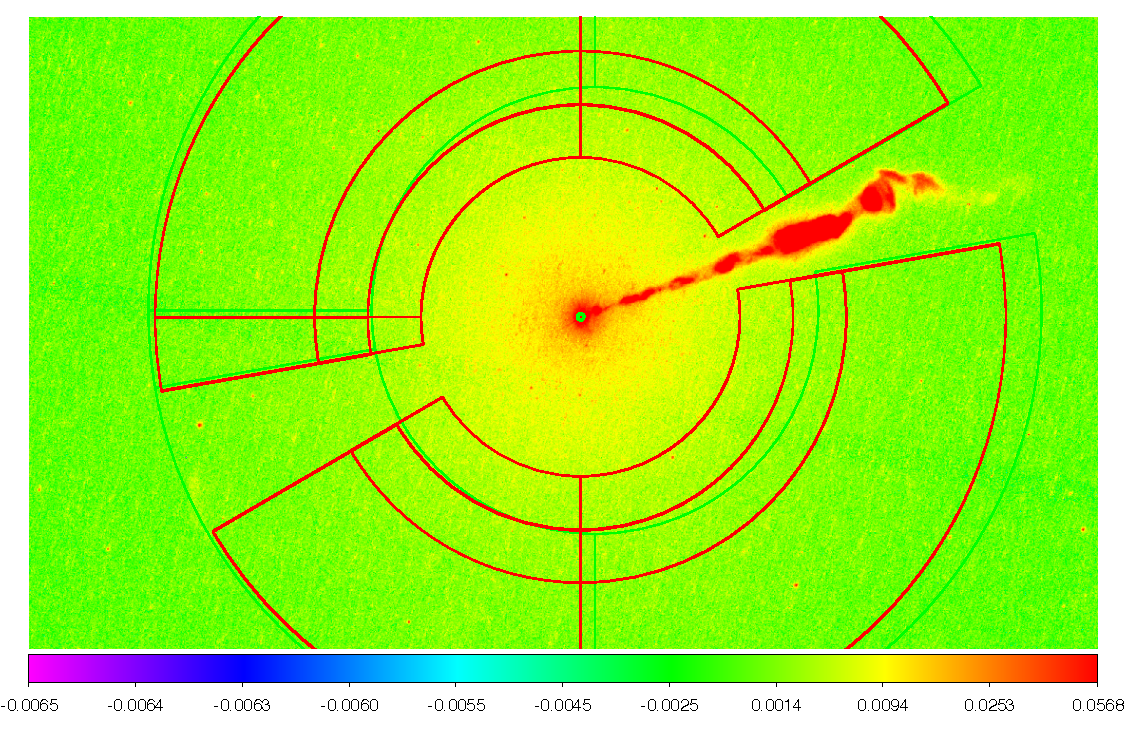
\includegraphics[width=\columnwidth]{ds9.pdf}
  \caption{Central region of M\,87 focussing on the AGN.  Several
    apertures to determine the centroid of the light are depicted.
    The two middle annuli lie from 9 to 15 arcseconds and 12 to 24
    arcseconds from the centre.  The inner apertures are circular and
    0.15 and 0.2 arcseconds in radius. The outermost aperture between
    24 and 36~arcseconds is not depicted.}
  \label{fig:M87}
\end{figure}

\section{Conclusions}

Both the calibration and observational analysis presented here can be
improved upon in several directions.  From the calibration standpoint,
we have consider just the force on the black hole and not the cotery
of stars in its immediate gravitational influence.  Moving the black
hole from the centre of the stellar system will also move these stars,
somewhat dilluting the Nordvedlt effect.  Of course in the simulations
that we did perform as the black hole oscillates about the centre of
mass of the stellar system, it carries the neighbouring stars with it,
but additional study is warranted where one would start the black hole
in the centre of the galaxy increase the differential acceleration,
say due to the effect of the small galaxy approxching the larger one,
and determine where the black hole ends up.

As we have mentioned earlier, there are more sophisticated ways to
determine the centre of the galaxy with isophotal fitting and by
considering measurements from several observations at several
wavelengths.  In priciple one could find tighter constraints on the
deviation of the black hole from the centre of the potential.  In the
case of M\,32 the existing constraints are just 0.5~arcseconds because
one has to link the radio coordinate system to the visual one.  These
could possibly be improved dramatically with further observations.
The visual core of M\,32 lies within 0.01~arcseconds of the centroid
of the outer isophotes of the galaxy, indicating that if the black
hole is coincident with the core, $|\eta_N|<0.06$, , competitive with the
results from pulsar timing \citep{Stairs:2005}.

Furthermore, the discovery of a supermassive black hole in one of the
other elliptical satellites of M\,31 could provide stronger
constraints from the M\,31 system.  However, the main uncertainty in
the constraints comes from the unknown geometry of the system as we
saw for M\,32 in particular so further information on the relative
distances of the various galaxies would yield better constraints on
the results.  Perhaps other interacting and nearly interacting
galaxies in the local Universe could also provide more information and
would statistically limit the violation of SEP in the motion of black
holes.

The constraint on SEP from the motion of black holes probes the SEP in
an essentially different limit that lunar ranging; however, the
technique outlined here could become competitive with the lunar
ranging results which now constrain $|\eta_N|<4.5 \times 10^{-4}$
\citep{Baess:1999}.  Improved astrometric measurements of the centre
of the potential of M\,87 and the location of the black hole could be
achieved with existing visual and UV data and the position of the
black hole could be constained further with radio inferemetry provided
the optical and radio astrometry could be tied together with
sufficient precision.  Relative astrometry with a precision $\sim
10^{-4}$ arcseconds can be achieved with Hubble photometry
\citep[e.g.][]{Heyl116397dyn}, a factor of one hundred better than
presented here, so constraints on $|\eta_N|$ of $10^{-3}$ could be
possible with supermassive black holes.  If microarcsecond astrometry
can be brought to bear \citep[e.g.][]{2011ApJ...735...57B} on M\,87,
then constaints on $\eta_N$ on the order of $10^{-4}$ might be possible.

This research is based on NASA/ESA Hubble Space Telescope observations
obtained at the Space Telescope Science Institute, which is operated
by the Association of Universities for Research in Astronomy
Inc. under NASA contract NAS5-26555 and accessed through the Hubble
Legacy Archive. These observations are associated with proposal
GO-11714 (PI: Bond) and GO-12989 (PI: Renzini).  This work was
supported by the Natural Sciences and Engineering Research Council of
Canada, the Canadian Foundation for Innovation and the British
Columbia Knowledge Development Fund.

\bibliography{weighbh}
\bibliographystyle{apj}


\label{lastpage}
\end{document}
